\chapter{Cryptographic Primitives \small{\textsf{DRAFT}}}

\section{Hash Functions}\index{Hash Function}

We already discussed the \emph{gossip protocol} that allows peer-to-peer nodes to exchange
objects on the network. Before exchanging an object, it is useful that the nodes can talk
\emph{about} these objects and ask each other whether they have a particular object. To
do this, it will be useful to give each object a unique identifier. We cannot use
increasing integers as identifiers, as these objects may be created in different parts of
the network and there is no global shared counter. We also cannot use a simple random
number as the identifier, as we want the identifier to be unfakeable: Given an identifier
we want to be able to check that the object really does correspond to the identifier.

For this, we will use \emph{cryptographically secure hash functions}\index{Hash function}. The hash function
is a function $H: \{0, 1\}^* \longrightarrow \{0, 1\}^\kappa$, where $\kappa$ is the
security parameter. As you can see, the hash function accepts \emph{any} string as input,
but \emph{always} returns a $\kappa$ bits long string. This makes it useful as a
\emph{compression} mechanism, as these identifiers are short ($\kappa$ will be $256$
bits in practice) and can be exchanged on the network prior to the actual objects.

\subsection*{Collision Resistance}

\import{./}{algorithms/alg.hash-collision}

Ideally, we would like each different object to correspond to exactly one hash
output:

\[
  \forall x_1, x_2: x_1 \neq x_2 \Rightarrow H(x_1) \neq H(x_1)
\]

However, this ideal goal is unattainable.
Because the hash function has \emph{unlimited} inputs and \emph{limited} outputs,
there will necessarily exist some \emph{collision} in which multiple inputs correspond
to the same output. To find a collision, we can start enumerating all the possible
inputs to the hash function starting at $0$ and going up to $2^\kappa$. If we have
not found a collision when we reach $2^\kappa - 1$, then this means that we have taken
up all of the possible $2^\kappa$ outputs. When we then evaluate the hash function on
the input $2^\kappa$, we will certainly find a collision. This process is shown in
Algorithm~\ref{alg.hash-collision}. Of course, as this function has to run through
$2^{2\kappa}$ combinations, its running time is exponential. The result that hash
functions must \emph{necessarily} have collisions stems from the Pigeonhole
Principle~\cite{liu}:

\begin{theorem}[Pigeonhole]
  Consider a function $f: A \longrightarrow B$. If $|A| > |B|$, then there must
  exist $x_1$ and $x_2$ such that $f(x_1) = f(x_2)$.
\end{theorem}

Instead, we will require that \emph{finding} such collisions is \emph{computationally}
difficult. We can define this in the form of the collision finding cryptographic game,
illustrated in Algorithm~\ref{alg.collision-game}.\index{Collision Resistance}

\import{./}{algorithms/alg.collision-game}

In this game, we ask the adversary to produce two different inputs $x_1$ and $x_2$
that have the same hash. Note that the hash function $H$ is different
for every value of $\kappa$ (while the code that produces the hash output for every
$\kappa$ is the same, it must take $\kappa$ into account when running), so we
denote it $H_\kappa$. It gives $\kappa$ bits of output. The adversary can have some
hard-coded collisions in her source code, but, if our hash function is secure, these won't work for
sufficiently large values of $\kappa$.

\subsection*{Gossiping with Hashes}

Collision resistance ensures that, if we are given a hash of something, we cannot
later be given something else that hashes to the same value. This makes hashes suitable
for use as identifiers of objects as we exchange them on the network. When gossiping
about objects, instead of sending a whole object to each of our peers, we can optimize
the process by advertising the ownership of an object through its hash. The hash of
an object used in this manner is called the \emph{objectid}. If the peer already knows
about this object, they can ignore our advertisement. If the peer has not seen the
object before, they can request the object through its objectid. Only at this point, we
send the full object to the peer. Upon receiving the object, the peer can verify that
it is indeed the requested object by hashing it and comparing it to the stored objectid.
Towards this purpose, each node must maintain a set of known objectids for quick lookup.

We now have a more complete understanding of how the gossiping protocol works:

\begin{enumerate}
  \item Node $A$ first becomes aware of a new object $O$, either by receiving it from a peer,
        or by generating it locally. Object $O$ has objectid $h = H(O)$, where the input to the
        hash function is a string-encoded versino of the object.
  \item $A$ advertises its knowledge of $O$ by sending a message
        indicating \emph{I have an object with objectid} $h$ to its peer $B$.
  \item $B$ receives the objectid $h$ and checks against its database whether it has already seen
        this object. Suppose that it has not. At this point, $B$ sends to $A$ a message
        requesting the contents of the object with objectid $h$.
  \item $A$ sends to $B$ the object $O$. Upon receiving $O$, the node $B$ can verify that
        $h = H(O)$, where $h$ is the requested objectid. This ensures that $A$ sent the
        correct object to $B$.
  \item In turn, $B$ advertises to \emph{its} peers that it now knows of an object with
        objectid $h$. It sends node $C$ a message indicating this.
  \item At this point, if $C$ has already received $O$ from $A$, it will not request
        the object from $B$. This is how the propagation in the gossiping algorithm stops.
\end{enumerate}

The node $B$ does not know whether $h$ was newly generated by $A$, or if $A$ is simply relaying.
This gives a modicum of anonymity: When a new object is first sent to us from an IP address,
we cannot deduce that the message is actually originating from that IP address.

\subsection*{Preimage resistance}

Hashes are also useful for allowing a party to \emph{commit} to a value. The party
reveals that hash, but not the object itself. Anyone who has the hash can verify that
the object is correct once the full object has been received, but it is useful that
this is not possible when seeing only the hash: It should be difficult to find the
\emph{preimage} of a hash given its image. Of course, the preimage of a hash can
be found by performing an exhaustive search in a similar fashion to
Algorithm~\ref{alg.hash-collision}, but this will take exponential time.
Naturally, we can define the property of \emph{preimage resistance} using a
cryptographic game.\index{Preimage Resistance}

\import{./}{algorithms/alg.preimage-game}

In this game, the challenger chooses a random $\kappa$-bit value as the input. This is denoted by
the $x \getsrandomly S$ symbol that indicates that an element $x$ is chosen uniformly at random
from the set $S$. Note here that to do this, the challenger, too, has access to randomness,
and so any probabilities are also taken with respect to this randomness.
The adversary is given $H(x)$ and would like to find $x$.
As there are other inputs that produce the same $H(x)$,
we ask her to produce some $x'$ (equal or different from $x$) that has the same hash value
as $x$.

\subsection*{Hash Security}

We can now define what it means for a hash function to be \emph{cryptographically secure}
or simply \emph{secure}.

\begin{definition}[Secure Hash Function]
  A hash function $H: \{0, 1\}^* \longrightarrow \{0, 1\}^\kappa$ is \emph{secure}
  if there is a negligible function \emph{negl} such that

  \begin{gather*}
    \forall PPT \mathcal{A}:\\
      \Pr[\textsf{collision-game}_{H,\mathcal{A}}(\kappa)] = 1] < \textsf{negl}
      \\\land\\
      \Pr[\textsf{preimage-game}_{H,\mathcal{A}}(\kappa)] = 1] < \textsf{negl}
  \end{gather*}
\end{definition}

\section{Hash Functions}
\quad We use hash functions to represent objects in the network. A hash function is a mathematical function that takes in an arbitrary string input and outputs a unique identifier of that string: $\mathcal{H}: \{0,1\}^* \rightarrow \{0,1\}^\kappa$.
In implementation, we use the SHA-256 hash function ($\kappa = 256$), meaning that the outputted address is of length 256. \\

\textbf{Gossiping strategy: }
\begin{enumerate}
    \item Upon learning of an object, advertise that you have it by its objectid, which is the hash of the object (meaning that we send it to all peers).
    \item Upon seeing an objectid, request it if you don't have it.
\end{enumerate}
Note: It is important that each object has a \textit{unique} identifier (one-to-one), since in the Gossip protocol, instead of sending an entire object, we signal ownership of it by sending its hash.\newline

However, since $|\kappa|$ may be $\leq *$, by the Pigeonhole Principle, $\exists x_1, x_2: H(x_1)=H(x_2)$. In other words, collisions exist because the input space is larger than the output space.

However, while collisions exist, they are hard to find which we will show.

To find a collision without polynomial time restriction, we can use a brute-force method: \\
\begin{algorithm}
\caption{Brute force collision finding}
\label{a'2}
\begin{algorithmic}[1]
\Function{Brute force collision finding}{$1^{\kappa}
$}
    \For {$i \in \{0,\dots,2^\kappa\}$}
    \For {$j \in \{i+1,\dots, 2^\kappa\}$}
    \If {$H(i) = H(j)$}
        \State \Return $(i,j)$
    \EndIf
    \EndFor
    \EndFor
\EndFunction
\end{algorithmic}
\end{algorithm}


The three properties we want to achieve are as follows:


\begin{algorithm}[H]
\caption{Collision Game}
\label{game:collision}
\begin{algorithmic}[1]
\Function{$\mathsf{COLL}_\mathcal{A}$}{$\kappa$}: \State $x, x' \leftarrow \mathcal{A}
(1^{\kappa})$    \Comment{Invoke adversary for both inputs}
\State \Return $x != x' \wedge H(x) = H(x')$
\EndFunction
\end{algorithmic}
\end{algorithm}

In Alg~\ref{game:collision}, we invoke the adversary for both inputs and return a collision. The adversary is successful if she returns $x\ne x'$ such that $H(x)=H(x')$.

\begin{algorithm}[H]
\caption{2nd-preimage Game}
\label{game:2pre}
\begin{algorithmic}[1]
\Function{$\mathsf{2PRE}_{\mathcal{A},H_\kappa}$}{$\kappa$}:
    \State $x_1 \getsrandomly \{0,1\}^{2\kappa+1}$
    \Let{x_2}{\mathcal{A}(x_1)}
    \State \Return $x_1 \neq x_2 \wedge H_\kappa(x_1) = H_\kappa(x_2)$
\EndFunction
\end{algorithmic}
\end{algorithm}

In Alg~\ref{game:2pre}, the adversary is given a randomly sampled $2\kappa+1$ bit input $x_1$ by the challenger. The adversary is successful if she can come up with an $x_2 \neq x_1$ that hashes to the same value as $x_1$, i.e. $H(x_1) = H(x_2)$.

\begin{algorithm}[H]
\caption{Preimage Game}
\label{game:pre}
\begin{algorithmic}[1]
\Function{$\mathsf{PRE}_{\mathcal{A},H_\kappa}$}{$\kappa$}:
    \State $x \getsrandomly \{0,1\}^{2\kappa+1}$
    \Let{y}{H_\kappa(x)}
    \Let{x'}{\mathcal{A}(y)}
    \State \Return $H(x') = y$
\EndFunction
\end{algorithmic}
\end{algorithm}

In Alg~\ref{game:pre}, the adversary is given the hash of a randomly sampled $2\kappa+1$ bit input and is successful if she can find an $x$ that hashes to the given hash.

A hash function is easy to compute but hard to invert, meaning that $x \rightarrow y$ is easy (polynomially computable) while the inversion of the hash function, $y \rightarrow x$, is hard.

\begin{theorem}
If $H$ is collision resistant, then $H$ is 2nd-preimage resistant. More formally, $\forall$ PPT (probabilistic polynomial time) $\mathcal{A}$: $Pr[\mathsf{2PRE}_{\mathcal{A}}(\kappa) = 1] \leq
negl(\kappa).$
\end{theorem}

\begin{proof}
For the sake of contradiction, suppose that $H$ is not 2nd-preimage resistant. Thus, there exists some adversary $\mathcal{A}$ such that $Pr[\mathsf{2PRE}_{\mathcal{A}}(\kappa)] = p$, where $p$ is non-negligible. We construct an adversary $\mathcal{A'}$ against Collision game (Alg.~\ref{a'}).

\begin{algorithm}
\caption{$\mathcal{A
}'$ adversary}
\label{a'}
\begin{algorithmic}[1]
\Function{$\mathcal{A
}'$}{$1^\kappa$}:
    \State $x_1 \leftarrow R \{0,1\}^{2\kappa+1}$
    \State $x_2 \leftarrow \mathcal{A}(x_1)$
    \State \textbf{return} $x_1, x_2$
\EndFunction
\end{algorithmic}
\end{algorithm}

$Pr[\mathsf{COLL}_{\mathcal{A}'}(\kappa)=1] = Pr[\mathsf{2PRE}_{\mathcal{A}}(\kappa)=1]$ = non-negligible
$\implies Pr[\mathsf{COLL}_\mathcal{A}'(\kappa)=1]$ is non-negligible.
This is a contradiction, hence, $H$ is 2-nd-preimage resistant.

\begin{figure}[H]
    \centering
    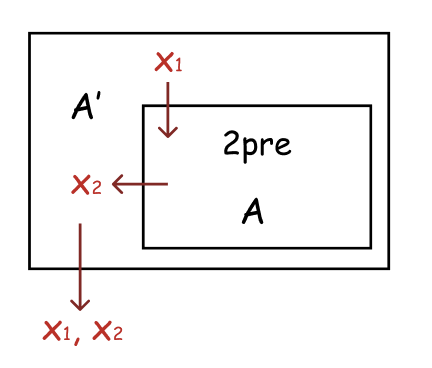
\includegraphics[scale=0.6]{figures/2pre.png}
    \caption{2nd-preimage game visualization: Follows \ref{a'} construction, in which $\mathcal{A}'$ produces $x_1$ and gives $x_1$ to $\mathcal{A}$. Then, $\mathcal{A}$ provides $x_2$ and $\mathcal{A}'$ returns $x_1, x_2$.}
    \label{fig:2pre_viz}
\end{figure}

\end{proof}

\begin{theorem}
% Hash $H$ has $\mathsf{2PRE}_\mathcal{A}$ security $\implies$ $H$ has $\mathsf{PRE}_\mathcal{A}$ security.
If $H$ is 2nd-preimage resistant, then $H$ is preimage resistant.
\end{theorem}

\begin{proof}
For the sake of contradiction, suppose that $H$ is not preimage resistant.  Then, there exists an  adversary against preimage. We construct $\mathcal{A}'$ against 2nd-preimage resistance \ref{a'2}.

\begin{algorithm}[H]
\caption{$\mathcal{A}'$ Construction}
\label{a'2}
\begin{algorithmic}[1]
\Function{$\mathcal{A}'$}{$1^\kappa$}:
    \State $x \leftarrow R \{0,1\}^{2\kappa+1}$
    \State $y \leftarrow H(x)$
    \State $x' \leftarrow \mathcal{A}(y)$
    \State \textbf{return} $x' \ne x_1 \wedge H(x')=H(x)$
\EndFunction
\end{algorithmic}
\end{algorithm}

\begin{figure}[H]
    \centering
    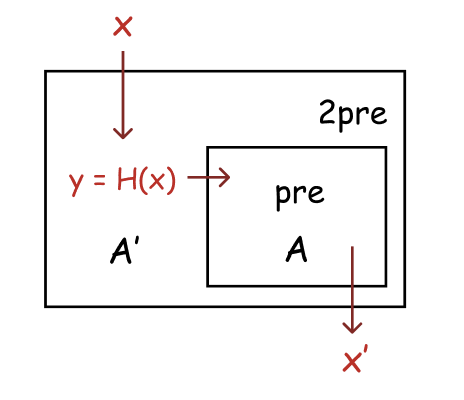
\includegraphics[scale=0.6]{figures/pre.png}
    \caption{Preimage game visualization: Follows \ref{a'2} construction, in which $\mathcal{A}'$ produces $y = H(x)$ given $x$. Then, give $y$ to $\mathcal{A}$ to produce $x'$.}
    \label{fig:pre_viz}
\end{figure}

We hope $x'\ne x$. Partition the input space into "boxes" ($y$: output value) containing dots ($x$: input value) that all hash to the same value. Sort boxes by their sizes (number of inputs) in ascending order, in which the larger boxes are on the left. The purpose of this is that we want to argue that it's harder to guess a dot in a larger box.

Next, we split into two halves of equal number of inputs ($2^{2\kappa}$ dots each half). It is impossible to have $< 2^\kappa$ dots in a "box" on the left half because then each box on the right half has $<2^\kappa$. There are $<2^\kappa$ boxes on the right half, each with $<2^\kappa$ dots, so the total dots in the right half is $<2^\kappa \cdot 2^\kappa = 2^{2\kappa} \implies $ there are $<2^{2\kappa}$ dots.
So, all the left-half boxes are "large".
The probability that we sampled an input on the left half = $\frac{1}{2}$ (sampling uniformly). The $y$ value of the box of our input will have $\geq 2^\kappa$. The adversary has no better strategy than guessing uniformly at random from the box. \\
Thus, there holds: $Pr[\mathsf{2PRE}_\mathcal{A}'(\kappa)] \geq Pr[\mathsf{PRE}_\mathcal{A}(\kappa)=1](\frac{1}{2})(1-2^{-\kappa})$
= non-negligible * constant * value close to 1 = non-negligible. So $Pr[\mathsf{2PRE}_\mathcal{A}'(\kappa)]$ is non-negligible. This implies that $\mathsf{2PRE}$ security is broken, in contradiction.
\end{proof}

\section{Transactions and Signatures}
\textbf{Verifiability of money}: If money is created correctly, money has verifiability property such as ownership validation. Here, we discuss a transfer of ownership.

In blockchain networks, a transaction is an entry in local state. Each node keeps a ledger, which is a recorded sequence of transactions ("tx"s). Ledgers are used to verify and update the system state, a record of the balances of all parties in the system, such that consensus across nodes is maintained.

Assume we have parties $A$, $B$, $C$, etc. Each party can have some sort of money and each party will share all financial information. An example of a transaction could be party $A$ saying "Give 5 units to party $B$." The following is an outline of ledger/transaction procedures:
\begin{enumerate}
    \item
    Initial system state: some distribution of money.
    \item
    Issue a tx by broadcasting
    \item
    Upon receiving a tx:
    \begin{enumerate}
        \item
        Check validity (source has enough money)
        \item
        Append to local ledger
    \end{enumerate}
    \item
    Read ledger to determine balances (system state)
\end{enumerate}

However, nobody should be able to issue transactions spending money from someone's else balance. Therefore, we need to authenticate transactions. One way to achieve it is by using digital signatures.

Digital signature scheme, Alg.~\ref{keys},  consists of three algorithms: key generation, signing and verifying algorithms.
% Key generation algorithms takes a security parameter as an input and outputs a pair of keys - public and private. Signing algorithms takes a message and a private key as an input and outputs a signature for the given message. Verifying algorithms takes as an input a public key, a message and a signature and outputs true if the given signature is valid.
\begin{algorithm}
\caption{Private and Public Keys: Signature Scheme}
\label{keys}
\begin{algorithmic}[1]
    \State $(pk, sk) \leftarrow Gen(1^\kappa)$
    \State $\sigma \leftarrow Sig(sk, m)$
    \State $Ver(pk, m, \sigma) \leftarrow \{\text{True}/\text{False}\}$
\end{algorithmic}
\end{algorithm}

An important property of digital signature scheme is \textbf{correctness}: $\forall m : (pk, sk) \leftarrow Gen(1^{\kappa}) : Ver(pk, m, Sig(sk, m)) = \text{True}$. In other words, for any message, we should be able to verify using a public key and $m$ such that $Ver() = True$. Transactions are happening between public keys and messages are signed with private key by the author, verified by other users via the author's public key. \\

For a signature scheme to be secure, it should be impossible for adversary to produce a valid signature without knowing a private key. More formally,
a security game for digital signatures is defined as follows in Alg~\ref{unforgable}:
\begin{algorithm}
\caption{Signatures are unforgable}
\label{unforgable}
\begin{algorithmic}[1]
\Function{$\mathsf{Forgery}_\mathcal{A}$}{$\kappa$}
    \State $M \leftarrow \emptyset$
    \State $(pk, sk) \leftarrow Gen(1^\kappa)$
    \State $\sigma, m \leftarrow \mathcal{A}^O(pk)$
    \State \textbf{return} $Ver(pk, m, \sigma) \wedge m \notin M$
\EndFunction
\end{algorithmic}
\end{algorithm}

We want to allow the adversary to have access to an oracle such that the adversary can choose an adversarial message. We use $M$ to track the set of messages requested by the adversary. We don't want to allow the adversary to simply invoke the oracle \ref{oracle} function and return a forged messaged outputted by $M$.

\textbf{Oracle}, that can be called by the adversary is defined in Alg.~\ref{oracle}.
\begin{algorithm}
\caption{Signatures are unforgable}
\label{oracle}
\begin{algorithmic}[1]
\Function{O}{$m'$}:
    \State $\sigma' \leftarrow Sig(sk, m')$
    \State $M \leftarrow M \cup \{m'\}$
    \State \textbf{return} $\sigma'$
\EndFunction
\end{algorithmic}
\end{algorithm}
